% ==========================================================
% 第5章 アフィン多様体と座標環
% ==========================================================
\chapter{アフィン多様体と座標環}
\label{ch:ch05}

\begin{chapterlead}
第4章では Hilbert の零点定理を通じて，代数的集合と根基イデアルの対応，および座標環 $k[X]$ を導入した．
本章ではこの対応を「対象」だけでなく「写像」のレベルにまで引き上げる．
すなわち，アフィン多様体 $X$ はその上の多項式関数のなす環 $k[X]$ によって完全に決まり，
さらに多様体の間の射 $X\to Y$ は $k$ 代数の準同型 $k[Y]\to k[X]$ と\emph{向きを逆にして}一対一に対応する．
この「幾何 $=$ 可換環の反対」という視点は，以後の局所化（第6章），次元と特異点（第7章），
そしてスキーム論（第12章）に至るまで本ノート全体を貫く基本原理である．

物理の言葉でいえば，「空間」を直接扱う代わりに「その上の観測量（関数）のなす代数」を扱う，という発想である．
古典力学の相空間を可観測量の Poisson 代数で記述すること，あるいは Gelfand 双対性や非可換幾何の思想と同じ方向を向いている．
\end{chapterlead}

本章を通じて $k$ は代数閉体とし，具体例では主に $k=\C$ を念頭におく．
多項式環を $k[x_1,\dots,x_n]$ と書き，$S\subset k[x_1,\dots,x_n]$ に対しその零点集合を $\Zero(S)$，
部分集合 $X\subset \A^n$ に対しその消滅イデアルを $\Ideal(X)$ と書く．

% ----------------------------------------------------------
\section{アフィン代数的集合の定義}
% ----------------------------------------------------------

\subsection{アフィン空間上の代数的集合}

まず舞台となる空間を確認する．
$n$ 次元アフィン空間 $\A^n=\A^n_k$ とは，集合としては $k^n$ そのものであるが，
「原点や線形構造を特別視しない」「多項式関数のみを関数として扱う」という気持ちを込めて別の記号で書く．
物理でいえば，ベクトル空間 $\R^4$ ではなく，原点を選んでいない Minkowski 時空（アフィン空間）を考えることに対応する．

\begin{mydef}{アフィン代数的集合}{ch05-alg-set}
部分集合 $S\subset k[x_1,\dots,x_n]$ に対し
\[
  \Zero(S)=\{\,p\in\A^n \mid \text{すべての } f\in S \text{ について } f(p)=0\,\}
\]
とおく．ある $S$ によって $X=\Zero(S)$ と書ける部分集合 $X\subset\A^n$ を\textbf{アフィン代数的集合}という．
\end{mydef}

$S$ が生成するイデアルを $(S)$ とすると $\Zero(S)=\Zero((S))$ であり，
Hilbert の基底定理により $(S)$ は有限生成である．
したがって任意のアフィン代数的集合は\emph{有限個}の多項式の共通零点として書ける：
\[
  X=\Zero(f_1,\dots,f_r).
\]

\begin{myex}{基本的な代数的集合}{ch05-basic-alg}
\begin{enumerate}
  \item $\A^n=\Zero(0)$，$\emptyset=\Zero(1)$．
  \item 1点 $p=(a_1,\dots,a_n)$ は $\Zero(x_1-a_1,\dots,x_n-a_n)$．
  \item 超曲面 $\Zero(f)$．例えば $\A^2$ の円 $\Zero(x^2+y^2-1)$，放物線 $\Zero(y-x^2)$，
        尖点曲線（cusp）$\Zero(y^2-x^3)$，結節曲線（node）$\Zero(y^2-x^2(x+1))$．
  \item 行列のなす空間 $M_n(k)\cong\A^{n^2}$ の中の $\SL_n=\Zero(\det-1)$，
        あるいは $\{A\mid A^{\mathsf T}A=1\}$ で定まる直交群 $O_n$．
\end{enumerate}
\end{myex}

\begin{figure}[H]
\centering
\begin{tikzpicture}[scale=0.85]
  % parabola
  \begin{scope}
    \draw[->,gray] (-1.8,0)--(1.8,0) node[right]{$x$};
    \draw[->,gray] (0,-0.5)--(0,2.6) node[above]{$y$};
    \draw[thick,blue,domain=-1.55:1.55,samples=60] plot (\x,{\x*\x});
    \node at (0,-1) {$y=x^2$};
  \end{scope}
  % cusp
  \begin{scope}[xshift=5cm]
    \draw[->,gray] (-0.8,0)--(2,0) node[right]{$x$};
    \draw[->,gray] (0,-1.9)--(0,1.9) node[above]{$y$};
    \draw[thick,red,domain=0:1.5,samples=60] plot ({\x*\x},{\x*\x*\x/1.2});
    \draw[thick,red,domain=0:1.5,samples=60] plot ({\x*\x},{-\x*\x*\x/1.2});
    \node at (0.6,-2.3) {$y^2=x^3$};
  \end{scope}
  % node
  \begin{scope}[xshift=10cm]
    \draw[->,gray] (-1.5,0)--(1.5,0) node[right]{$x$};
    \draw[->,gray] (0,-1.9)--(0,1.9) node[above]{$y$};
    \draw[thick,teal,domain=-1.3:1.3,samples=80] plot ({\x*\x-1},{\x*(\x*\x-1)});
    \node at (0,-2.3) {$y^2=x^2(x+1)$};
  \end{scope}
\end{tikzpicture}
\caption{$\A^2_\R$ に描いた平面曲線の実点．左から放物線，尖点曲線，結節曲線．}
\label{fig:ch05-curves}
\end{figure}

\subsection{アフィン代数的集合の基本性質}

第3章・第4章で見たように，零点集合をとる操作は次の性質をもつ．

\begin{myprop}{零点集合の基本性質}{ch05-zero-basic}
$S,T\subset k[x_1,\dots,x_n]$，$\{S_\lambda\}_\lambda$ を部分集合の族，$I,J$ をイデアルとする．
\begin{enumerate}
  \item $S\subset T$ ならば $\Zero(T)\subset\Zero(S)$．
  \item $\Zero(I)\cup\Zero(J)=\Zero(IJ)=\Zero(I\cap J)$．
  \item $\bigcap_\lambda \Zero(S_\lambda)=\Zero\bigl(\bigcup_\lambda S_\lambda\bigr)$．
\end{enumerate}
\end{myprop}

\begin{proof}
(1) と (3) は定義から明らか．(2) について，$IJ\subset I\cap J\subset I$ より
$\Zero(I)\cup\Zero(J)\subset\Zero(I\cap J)\subset\Zero(IJ)$．
逆に $p\notin\Zero(I)\cup\Zero(J)$ なら $f(p)\ne0$ なる $f\in I$ と $g(p)\neq 0$ なる $g\in J$ がとれ，
$fg\in IJ$ かつ $(fg)(p)\ne0$ なので $p\notin\Zero(IJ)$．
\end{proof}

したがってアフィン代数的集合の全体は有限和と任意個の共通部分で閉じ，$\emptyset,\A^n$ を含む．
これらを閉集合とする位相が \textbf{Zariski 位相}である（第3章）．
アフィン代数的集合 $X\subset\A^n$ には常に $\A^n$ からの相対位相を入れる．
Zariski 位相は通常の（Euclid）位相よりはるかに粗く，例えば $\A^1$ の真の閉集合は有限集合だけである．
これは「多項式の零点は孤立しているか全体か」という代数の剛性を反映しており，
物理的直感とずれる最初のポイントである．

また $\A^n$ は Noether 位相空間である：閉集合の降鎖 $X_1\supset X_2\supset\cdots$ は必ず停留する．
実際 $\Ideal(X_1)\subset\Ideal(X_2)\subset\cdots$ は Noether 環 $k[x_1,\dots,x_n]$ のイデアルの昇鎖であり停留し，
$X_i=\Zero(\Ideal(X_i))$ だからである．

\subsection{既約アフィン代数的集合}

\begin{mydef}{既約性}{ch05-irred}
空でない位相空間 $X$ が\textbf{既約}であるとは，$X=X_1\cup X_2$（$X_1,X_2$ は閉集合）と書けるならば
$X=X_1$ または $X=X_2$ となることをいう．
\end{mydef}

既約な空間では空でない開集合は必ず稠密であり，空でない開集合どうしは必ず交わる．
Euclid 位相では1点以外の Hausdorff 空間は既約になりえないので，既約性は Zariski 位相特有の概念である．

\begin{myprop}{既約性と素イデアル}{ch05-irred-prime}
アフィン代数的集合 $X\subset \A^n$ が既約であるための必要十分条件は，$\Ideal(X)$ が素イデアルであることである．
\end{myprop}

これは第3章の定理\ref{thm:ch03-irred-prime}の再掲であり，証明もそちらを参照されたい
（要点は，$fg\in\Ideal(X)$ なら $X=(X\cap\Zero(f))\cup(X\cap\Zero(g))$ と閉集合に分解されること）．

Noether 性から次の分解定理が従う．

\begin{mythm}{既約成分分解}{ch05-irred-decomp}
任意のアフィン代数的集合 $X$ は有限個の既約閉集合の和 $X=X_1\cup\cdots\cup X_r$ として書ける．
$i\ne j$ について $X_i\not\subset X_j$ を課せばこの分解は順序を除いて一意であり，各 $X_i$ を $X$ の\textbf{既約成分}という．
\end{mythm}

証明は第3章の定理\ref{thm:ch03-irred-decomp}で与えた（存在は Noether 性による極小反例の議論，一意性は既約性から $X_i\subset Y_j\subset X_l$ となることによる）．

代数的にはこれは根基イデアルの準素分解 $\Ideal(X)=\p_1\cap\cdots\cap\p_r$（$\p_i=\Ideal(X_i)$ は極小素イデアル）に対応する．

\begin{myex}{既約成分}{ch05-components}
$\Zero(xy)\subset\A^2$ は二つの座標軸 $\Zero(x)\cup\Zero(y)$ に分解し，$(xy)=(x)\cap(y)$．
また $\Zero(xz,yz)\subset\A^3$ は $xy$ 平面 $\Zero(z)$ と $z$ 軸 $\Zero(x,y)$ の和であり，
既約成分の次元が異なりうることがわかる．一方，結節曲線 $\Zero(y^2-x^2(x+1))$ は原点で自己交差するが，
$y^2-x^2(x+1)$ は既約多項式なので曲線としては既約である．「見た目に2本の枝がある」ことと「既約成分が2つ」は別の概念である
（枝は局所的な概念であり，第6章・第7章で局所環を用いて扱う）．
\end{myex}

\subsection{アフィン代数的集合と方程式系}

アフィン代数的集合とは，要するに「多項式連立方程式の解集合」である．
ただし同じ解集合が多くの異なる方程式系から得られる点に注意が必要である．例えば
\[
  \Zero(x)=\Zero(x^2)=\Zero(x, xy)\subset \A^2 .
\]
方程式系 $f_1=\cdots=f_r=0$ の情報のうち，解集合 $X$ に依存する部分はイデアル $(f_1,\dots,f_r)$ の根基のみである：
零点定理（第4章）により
\[
  \Ideal(\Zero(f_1,\dots,f_r))=\sqrt{(f_1,\dots,f_r)} .
\]
すなわち
\[
  \{\text{アフィン代数的集合 } X\subset\A^n\}\ \overset{1:1}{\longleftrightarrow}\ \{\text{根基イデアル } I\subset k[x_1,\dots,x_n]\}
\]
であり，この下で既約集合は素イデアルに，点は極大イデアルに対応する．

方程式系を「同値な変形」で書き換えても解集合は変わらない．Gröbner 基底による消去や，変数変換
$x_i\mapsto x_i+(\text{他の変数の多項式})$ はこの意味の書き換えである．
一方，$x=0$ と $x^2=0$ の違い（重複度・無限小の情報）は古典的な代数的集合では失われる．
この情報を保持するのがスキーム論であり，第12章で扱う．

\begin{physbox}[拘束系と代数的集合]
解析力学で，相空間 $T^*Q$ 上の拘束条件 $\phi_a(q,p)=0$ が多項式で与えられるとき，拘束面はアフィン代数的集合である．
Dirac の議論では「弱い等号」$F\approx G$（拘束面上で等しい）が重要であったが，
これはまさに $F-G\in\Ideal(\text{拘束面})$ を意味する．
拘束条件 $\phi_a$ が生成するイデアルが根基でないとき（例えば $\phi=p^2$ のような拘束），
$\phi$ そのものではなく根基の生成元を用いないと拘束面上の関数がうまく記述できない，という
Dirac の「正則性条件」の問題が生じる．これは $\Zero(I)$ と $\sqrt I$ の区別そのものである．
\end{physbox}

\exprob{prob:ch05-1-1}
$X=\Zero(x^2-yz,\ xz-x)\subset\A^3$ の既約成分（問\ref{prob:ch03-9}）それぞれの消滅イデアルを書き，それらの共通部分が $\Ideal(X)$ に等しいことを確かめよ．

\exprob{prob:ch05-1-2}
$\A^1$ の Zariski 位相において，無限部分集合は稠密であることを示せ．また $\A^2$ の Zariski 位相は
$\A^1\times\A^1$ の積位相と一致しないことを示せ．

% ----------------------------------------------------------
\section{アフィン多様体}
% ----------------------------------------------------------

\subsection{アフィン多様体の定義}

\begin{mydef}{アフィン多様体}{ch05-aff-var}
既約なアフィン代数的集合 $X\subset\A^n$ を\textbf{アフィン多様体}という．
同値な言い換えとして，$\Ideal(X)$ が素イデアルであるアフィン代数的集合のことである．
\end{mydef}

\begin{note}
文献によっては既約性を課さず，アフィン代数的集合そのもの（に後述の構造を合わせたもの）をアフィン多様体と呼ぶ．
本ノートでは既約なものをアフィン多様体と呼ぶが，本章の主要な結果（射と環準同型の対応，反変同値）は
既約性を仮定せずに成り立つので，必要に応じて「アフィン代数的集合」の場合も併記する．
\end{note}

「多様体」という言葉に引っ張られて，微分幾何の多様体（局所的に $\R^n$ と同相）を想像してはいけない．
代数多様体は特異点（cusp や node）を許す．特異点を持たない多様体を\emph{非特異}あるいは\emph{滑らか}な多様体と呼び，
第7章で Jacobian 判定法を用いて詳しく調べる．$k=\C$ のとき非特異なアフィン多様体は，
Euclid 位相で複素多様体になる．

\subsection{既約性とアフィン多様体}

なぜ既約性を課すのか．理由は主に次の3点である．
\begin{enumerate}
  \item \textbf{次元が well-defined になる．} 既約成分ごとに次元が異なりうる（例 \ref{ex:ch05-components}）．
        既約ならば次元は「どの点でも同じ」と期待でき，実際そうなる（第7章）．
  \item \textbf{関数体が定まる．} 既約なら座標環 $k[X]$ は整域であり（命題 \ref{prop:ch05-domain}），
        商体 $k(X)=\Frac k[X]$（関数体）がとれる．これは有理写像・双有理幾何（第10章）の基礎である．
  \item \textbf{一致の定理が成り立つ．} 既約な $X$ の上では，空でない開集合上で一致する二つの多項式関数は $X$ 全体で一致する．
\end{enumerate}

(3) を確かめておこう．$U\subset X$ を空でない開集合，$f\in k[X]$ が $U$ 上 $0$ とする．
$X=\Zero_X(f)\cup(X\setminus U)$ は閉集合の和で，$X\setminus U\neq X$ なので既約性から $X=\Zero_X(f)$，すなわち $f=0$．
これは正則（holomorphic）関数に対する一致の定理の類似であり，代数的関数の「剛性」を表している．
滑らかな関数が台をコンパクトにとれる（bump function が存在する）のとは対照的で，第6章の\ref{sec:ch06-phys}節で場の理論の局所性と比較する際に重要になる．

\subsection{アフィン多様体の例}

\begin{myex}{アフィン多様体の例}{ch05-var-examples}
\begin{enumerate}
  \item $\A^n$ 自身：$\Ideal(\A^n)=(0)$ は素イデアル．
  \item 既約多項式 $f$ の定める超曲面 $\Zero(f)$：$k[x_1,\dots,x_n]$ は UFD なので $(f)$ は素イデアル．
        放物線，円（$\mathrm{char}\,k\neq 2$），尖点曲線，結節曲線はいずれもアフィン多様体である．
  \item 線形部分空間（の平行移動）：1次式で生成されるイデアルは素イデアル．
  \item ねじれ3次曲線 $C=\{(t,t^2,t^3)\mid t\in k\}=\Zero(y-x^2,\ z-x^3)\subset\A^3$．
        $k[x,y,z]/(y-x^2,z-x^3)\cong k[x]$ は整域．
  \item $\SL_n=\Zero(\det-1)\subset\A^{n^2}$．$\det-1$ は既約多項式であることが示せる．
  \item 二次錐面 $\Zero(xy-z^2)\subset\A^3$．$xy-z^2$ は既約．
\end{enumerate}
\end{myex}

\begin{myex}{既約でない例}{ch05-nonirr}
$O_2=\{A\in M_2(k)\mid A^{\mathsf T}A=1\}$ を考える．
行列式は $\pm1$ をとり，$O_2=SO_2\sqcup(O_2\cap\Zero(\det+1))$ と二つの既約成分に分解する．
物理でおなじみの「回転」と「反転を含む変換」の2成分であり，Lie 群の連結成分の分解が既約成分分解として現れている．
\end{myex}

\subsection{多様体と代数的集合の関係}

既約成分分解（定理 \ref{thm:ch05-irred-decomp}）により，任意のアフィン代数的集合は有限個のアフィン多様体の和である．
したがって多くの問題は既約な場合に帰着できる．
対応をまとめると次のようになる．
\begin{center}
\renewcommand{\arraystretch}{1.3}
\begin{tabular}{c|c}
幾何 & 代数（$k[x_1,\dots,x_n]$ のイデアル）\\ \hline
アフィン代数的集合 $X$ & 根基イデアル $\Ideal(X)$\\
アフィン多様体（既約） & 素イデアル\\
点 & 極大イデアル\\
既約成分分解 & 極小素イデアルによる表示 $\sqrt I=\p_1\cap\dots\cap\p_r$
\end{tabular}
\end{center}

注意すべきは，この表は $\A^n$ への\emph{埋め込み}を固定した記述だという点である．
放物線 $\Zero(y-x^2)\subset\A^2$ と直線 $\A^1$ は「同じもの」と思いたいが，イデアルは違う環の中にある．
埋め込みに依らない本質的な情報を取り出すのが座標環であり，次節以降の主題である．

\exprob{prob:ch05-2-1}
$X=\Zero(xy-z^2)\subset \A^3$ がアフィン多様体であることを示せ（$xy-z^2$ が既約であることを確かめよ）．
また $X$ の座標環において $\bar z^2=\bar x\bar y$ は $\bar z$ の既約元への分解と $\bar x,\bar y$ への分解を与え，
$k[X]$ は UFD でないことを示せ（$\bar x,\bar y,\bar z$ が $k[X]$ で既約元であることを次数を用いて示してよい）．

% ----------------------------------------------------------
\section{座標環の構成}
% ----------------------------------------------------------

\subsection{多項式関数}

$X\subset \A^n$ をアフィン代数的集合とする．
多項式 $F\in k[x_1,\dots,x_n]$ は写像 $\A^n\to k$ を定めるので，$X$ に制限して関数 $F|_X:X\to k$ が得られる．

\begin{mydef}{多項式関数}{ch05-poly-func}
写像 $f:X\to k$ が\textbf{多項式関数}であるとは，ある $F\in k[x_1,\dots,x_n]$ が存在して $f=F|_X$ となることをいう．
$X$ 上の多項式関数全体を $k[X]$ と書く．
\end{mydef}

$k[X]$ は点ごとの和と積で可換環となり，定数関数を通じて $k$ を含むので $k$ 代数である．
集合 $X$ 上の $k$ 値関数全体のなす $k$ 代数 $\mathrm{Map}(X,k)$ の部分代数であることに注意しよう．
とくに，$k[X]$ の元は「値」によって決まる関数である．
この点が，後に第12章で扱うスキーム（環の元が値だけでは決まらない）との大きな違いである．

物理では「空間上の可観測量（observable）」に相当する．
$X$ が拘束面なら，$k[X]$ は拘束面上の物理量の代数（Dirac 括弧以前の可換代数）である．

\subsection{多項式関数の同値性}

異なる多項式が $X$ 上で同じ関数を定めることがある．例えば放物線 $X=\Zero(y-x^2)$ 上で $y$ と $x^2$ は同じ関数である．
いつ同じになるかは明らかである：
\[
  F|_X=G|_X\iff (F-G)(p)=0\ (\forall p\in X)\iff F-G\in\Ideal(X).
\]
すなわち「$X$ 上で等しい」という同値関係は，イデアル $\Ideal(X)$ を法とする合同関係そのものである．

ここで用いるイデアルが $\Ideal(X)$ であって，$X$ を定義するのに用いた方程式のイデアル $I=(f_1,\dots,f_r)$ ではないことに注意する．
$I\subsetneq \Ideal(X)=\sqrt{I}$ のとき，$I$ を法とする合同は $X$ 上の関数としての等しさよりも細かい．
例えば $X=\Zero(x^2)\subset\A^1$ は原点 $\{0\}$ であり，$x$ は $X$ 上で関数として $0$ だが $x\notin(x^2)$．
（$k[x]/(x^2)$ はいわば「無限小の厚みをもった点」の関数環であり，第12章のスキームで重要な役割を果たす．）

\subsection{座標環の構成}

以上をまとめると次の定理になる．

\begin{myprop}{座標環の表示}{ch05-coord-ring}
制限写像 $\rho: k[x_1,\dots,x_n]\to k[X]$，$F\mapsto F|_X$ は全射な $k$ 代数準同型で，核は $\Ideal(X)$ である．したがって
\[
  k[X]\cong k[x_1,\dots,x_n]/\Ideal(X).
\]
\end{myprop}

\begin{proof}
$\rho$ が $k$ 代数準同型であることは，関数の和・積が点ごとに定義されていることから従う．
全射性は多項式関数の定義そのもの．核が $\Ideal(X)$ であることは前小節で見た．準同型定理より主張を得る．
\end{proof}

\begin{mydef}{座標環}{ch05-coord-ring-def}
$k[X]=k[x_1,\dots,x_n]/\Ideal(X)$ を $X$ の\textbf{座標環}（アフィン座標環）という．
$x_i$ の像を $\bar x_i$ と書き，\textbf{座標関数}と呼ぶ．
\end{mydef}

二つの記述 ―― 「関数のなす環」と「多項式環の商」 ―― は同じものの二つの顔である．
前者は埋め込み $X\subset\A^n$ によらない内在的な記述であり（関数 $X\to k$ の集合として定まる），
後者は計算に便利な具体的表示である．$k[X]$ は $\bar x_1,\dots,\bar x_n$ によって $k$ 代数として生成される．

\begin{figure}[H]
\centering
\begin{tikzcd}[column sep=large,row sep=large]
  k[x_1,\dots,x_n] \arrow[r,"\rho",two heads] \arrow[d,two heads] & k[X]\subset \mathrm{Map}(X,k)\\
  k[x_1,\dots,x_n]/\Ideal(X) \arrow[ru,"\cong"'] &
\end{tikzcd}
\caption{座標環の二つの記述．}
\end{figure}

\subsection{座標環と定義イデアル}

$X=\Zero(I)$ と書いたとき，商環 $k[x_1,\dots,x_n]/I$ と座標環 $k[X]$ の関係は次の通りである．

\begin{myprop}{}{ch05-coord-def-ideal}
$I\subset k[x_1,\dots,x_n]$ をイデアル，$X=\Zero(I)$ とする．自然な全射
\[
  k[x_1,\dots,x_n]/I\twoheadrightarrow k[X]
\]
の核は $\sqrt I/I$，すなわち $k[x_1,\dots,x_n]/I$ の冪零元全体のなすイデアル（冪零根基）である．
とくに，この全射が同型であることと $I$ が根基イデアルであることは同値である．
\end{myprop}

\begin{proof}
零点定理より $\Ideal(X)=\sqrt I$ なので核は $\sqrt I/I$．$\bar F\in k[x]/I$ が冪零 $\iff$ ある $m$ で $F^m\in I$ $\iff F\in\sqrt I$．
\end{proof}

\begin{myex}{定義イデアルが根基でない場合}{ch05-nonrad}
$I=(y^2,\ y-x^2)\subset k[x,y]$ とする．$\Zero(I)$ は放物線と二重直線 $y^2=0$（$x$ 軸）の交わりであり，集合としては原点のみである．
$k[x,y]/I\cong k[x]/(x^4)$ は4次元の $k$ ベクトル空間で，$\bar x$ は冪零．
一方 $k[\Zero(I)]=k[\{0\}]=k$．差の3次元は，放物線が $x$ 軸に原点で接しており（交点重複度 $2$），さらに $x$ 軸を二重に数えている（放物線と二重直線 $y^2=0$ の交点重複度は $2\times2=4$，第9章参照）という情報を担っている．
\end{myex}

\subsection{座標環の具体例}

第4章の例\ref{ex:ch04-coord-examples}で見た例を，同型写像を明示して再確認しておく．

\begin{myex}{座標環の計算}{ch05-coord-examples}
\begin{enumerate}
  \item $k[\A^n]=k[x_1,\dots,x_n]$，$k[\text{点}]=k$．
  \item 放物線 $X=\Zero(y-x^2)$：$k[x,y]/(y-x^2)\to k[t]$，$x\mapsto t$，$y\mapsto t^2$ は同型．よって $k[X]\cong k[t]$．
  \item 双曲線 $H=\Zero(xy-1)$：$k[x,y]/(xy-1)\cong k[t,t^{-1}]$（Laurent 多項式環），$x\mapsto t,\ y\mapsto t^{-1}$．
  \item 尖点曲線 $C=\Zero(y^2-x^3)$：$k[x,y]/(y^2-x^3)\cong k[t^2,t^3]\subset k[t]$．
        実際 $x\mapsto t^2,\ y\mapsto t^3$ は well-defined で，像は $k[t^2,t^3]=\{\sum a_it^i\mid a_1=0\}$．
        単射性は，$k[x,y]/(y^2-x^3)$ の任意の元が $a(x)+b(x)y$ と一意に書け，その像 $a(t^2)+b(t^2)t^3$ は偶数次と奇数次に分かれることから従う．
  \item 二つの座標軸 $X=\Zero(xy)$：$k[X]=k[x,y]/(xy)$．$\bar x\bar y=0$ で $\bar x,\bar y\neq0$ なので零因子をもつ．
  \item 円 $\Zero(x^2+y^2-1)$（$k=\C$）：$u=x+iy,\ v=x-iy$ とおくと $uv=1$ となり，双曲線と同型．$k[X]\cong\C[t,t^{-1}]$．
\end{enumerate}
\end{myex}

(6) は興味深い．実数体上では円（コンパクト）と双曲線（非コンパクト）は全く違うが，複素化すると同じものになる．
複素円 $\{x^2+y^2=1\}\subset\C^2$ は $\C^\times$ と同型であり，実の円 $S^1=U(1)$ は $\C^\times$ の中の $|t|=1$ の部分にすぎない．

\begin{physbox}[$U(1)$ とその複素化]
$U(1)$ の複素化は $\C^\times=\GL_1(\C)$ であり，代数群としては $\Zero(xy-1)\subset\A^2$，座標環は $\C[t,t^{-1}]$ である．
$U(1)$ の既約表現 $e^{in\theta}$（$n\in\Z$）が座標環の基底 $t^n$ に対応している．
Fourier 級数の「三角多項式」の環は，まさにこの座標環である．
一般に，コンパクト Lie 群 $G$ の複素化 $G_\C$ は代数群（アフィン多様体）となり，その座標環 $\C[G_\C]$ は
Peter--Weyl の定理により $\bigoplus_{V}V^*\otimes V$（$V$ は既約表現）と分解する．
\end{physbox}

\exprob{prob:ch05-3-1}
ねじれ3次曲線 $C=\Zero(y-x^2,\ z-x^3)\subset\A^3$ を考える（$k[C]\cong k[t]$ は問\ref{prob:ch04-8}で示した）．
$J=(xz-y^2,\ y-x^2)$ とするとき，$\Zero(J)$ を既約分解し，$\Zero(J)\supsetneq C$ であること（したがって $J\ne\Ideal(C)$）を示せ．
また $C$ を切り出すには $xz-y^2,\ y-x^2$ にどのような方程式を追加すればよいか答えよ．

% ----------------------------------------------------------
\section{座標環の性質}
% ----------------------------------------------------------

\subsection{座標環の有限生成性}

\begin{myprop}{座標環は有限生成被約 $k$ 代数}{ch05-fg-reduced}
アフィン代数的集合 $X$ の座標環 $k[X]$ は次を満たす．
\begin{enumerate}
  \item $k$ 代数として有限生成である．
  \item 被約である，すなわち $0$ 以外の冪零元をもたない．
\end{enumerate}
逆に，有限生成被約 $k$ 代数 $A$ は，あるアフィン代数的集合 $X$ の座標環と $k$ 代数として同型である．
\end{myprop}

\begin{proof}
(1) $k[X]$ は座標関数 $\bar x_1,\dots,\bar x_n$ で生成される．
(2) $f\in k[X]$ が $f^m=0$ を満たせば，各点 $p$ で $f(p)^m=0$，体 $k$ は整域なので $f(p)=0$．よって $f=0$．
（イデアルの言葉では，$\Ideal(X)$ が根基イデアルであることと同じである．）

逆に $A$ が $a_1,\dots,a_n$ で生成されるとすると，全射 $\pi:k[x_1,\dots,x_n]\to A$，$x_i\mapsto a_i$ がある．
$I=\Ker\pi$ とおけば $A\cong k[x_1,\dots,x_n]/I$．$A$ が被約であることは $I$ が根基であることと同値である
（$F^m\in I\Rightarrow \pi(F)^m=0\Rightarrow\pi(F)=0\Rightarrow F\in I$）．
$X=\Zero(I)$ とすれば零点定理より $\Ideal(X)=\sqrt I=I$，よって $k[X]\cong A$．
\end{proof}

この命題の後半で，零点定理（$k$ が代数閉体であること）が本質的に使われている．
例えば $k=\R$ で $A=\R[x]/(x^2+1)\cong\C$ は有限生成被約 $\R$ 代数だが，$\Zero_\R(x^2+1)=\emptyset$ であり，
実点の上の関数環としては実現できない．

$A$ の生成元のとり方は一意ではない．生成元を変えると $X$ は別の $\A^m$ の中に実現されるが，
後で見るように（\ref{sec:ch05-ring-geom} 節）それらはすべて互いに同型な多様体である．

\subsection{座標環と整域}

\begin{myprop}{既約 $\iff$ 座標環が整域}{ch05-domain}
アフィン代数的集合 $X$ について次は同値である．
\begin{enumerate}
  \item $X$ は既約である（すなわちアフィン多様体である）．
  \item $\Ideal(X)$ は素イデアルである．
  \item $k[X]$ は整域である．
\end{enumerate}
\end{myprop}

\begin{proof}
(1)$\iff$(2) は命題 \ref{prop:ch05-irred-prime}．(2)$\iff$(3) は「$R/\p$ が整域 $\iff$ $\p$ が素イデアル」という一般論である．
\end{proof}

(3) の幾何的意味を直接見ておくと理解が深まる．$X=X_1\cup X_2$ が真の分解なら，
$f$ を「$X_1$ 上で $0$，$X_2$ 上で $0$ でない」関数，$g$ をその逆とすると，$fg=0$ だが $f,g\ne0$ である．
座標軸 $\Zero(xy)$ では $f=\bar x$，$g=\bar y$ がそれである（図 \ref{fig:ch05-zero-div}）．
零因子は「別々の成分に台をもつ関数」の存在を意味する．

\begin{figure}[H]
\centering
\begin{tikzpicture}[scale=0.9]
  \draw[very thick,blue] (-2,0)--(2,0) node[right]{$\Zero(y)$：ここで $\bar y=0$};
  \draw[very thick,red] (0,-1.5)--(0,1.5) node[above]{$\Zero(x)$：ここで $\bar x=0$};
  \fill (0,0) circle (2pt);
\end{tikzpicture}
\caption{$\Zero(xy)$ 上で $\bar x\bar y=0$ だが $\bar x,\bar y\neq0$．}
\label{fig:ch05-zero-div}
\end{figure}

\subsection{座標環と既約性}

以上から，\emph{アフィン多様体の座標環は有限生成な整域 $k$ 代数}であり，逆に有限生成整域 $k$ 代数はアフィン多様体の座標環である．
既約成分分解は座標環の言葉では次のように表される．
$X=X_1\cup\cdots\cup X_r$ を既約成分分解，$\p_i=\Ideal(X_i)/\Ideal(X)\subset k[X]$ とすると，
$\p_1,\dots,\p_r$ はちょうど $k[X]$ の極小素イデアルであり，
\[
  \p_1\cap\cdots\cap\p_r=0,\qquad k[X]\hookrightarrow \prod_{i=1}^r k[X_i]
\]
が成り立つ（$f\mapsto(f|_{X_1},\dots,f|_{X_r})$ が単射であることは明らか）．
ただしこれは一般には全射ではない：$X=\Zero(xy)$ では $k[X]\to k[x]\times k[y]$ の像は
$\{(a(x),b(y))\mid a(0)=b(0)\}$ であり，「二つの成分が原点で貼り合わされている」ことを表している．
既約成分が交わらない場合に限りこの写像は同型になる（中国剰余定理）．

\subsection{座標環による幾何学的情報の表現}

座標環には $X$ の幾何学的情報がすべて含まれている．第4章で見た対応を $k[X]$ の言葉で言い直すと：

\begin{myprop}{座標環のイデアルと $X$ の部分集合}{ch05-ideal-corr}
アフィン代数的集合 $X$ に対し，$J\subset k[X]$ をイデアルとして $\Zero_X(J)=\{p\in X\mid f(p)=0\ \forall f\in J\}$，
$Y\subset X$ に対し $\Ideal_X(Y)=\{f\in k[X]\mid f|_Y=0\}$ とおく．このとき
\[
  \{X\text{ の閉部分集合}\}\overset{1:1}{\longleftrightarrow}\{k[X]\text{ の根基イデアル}\}
\]
であり，既約閉部分集合は素イデアルに，点は極大イデアルに対応する．
点 $p\in X$ に対応する極大イデアルは $\m_p=\{f\in k[X]\mid f(p)=0\}$ であり，$k[X]/\m_p\cong k$（$f\mapsto f(p)$）．
\end{myprop}

\begin{proof}[証明の概略]
$k[X]=k[x]/\Ideal(X)$ のイデアルは $\Ideal(X)$ を含む $k[x]$ のイデアルと一対一に対応し，この対応は根基性・素性・極大性を保つ．
あとは $\A^n$ での対応（第4章）を $X$ に制限すればよい．
\end{proof}

すなわち $X$ は集合として $k[X]$ の極大イデアル全体 $\mathrm{Max}\,k[X]$ と同一視でき，
Zariski 位相も $k[X]$ から復元できる．関数 $f\in k[X]$ の点 $p$ での値は「$f$ の $k[X]/\m_p\cong k$ での像」である．
こうして\emph{空間 $X$ を忘れて環 $k[X]$ だけから $X$ を再構成できる}．
極大イデアルだけでなく素イデアル全体を点とみなすのが $\Spec$ であり，第12章で導入する．

\begin{physbox}[状態と可観測量]
量子力学・古典力学のいずれでも，「状態」は可観測量の代数 $\mathcal A$ 上の線形汎関数（期待値）$\omega:\mathcal A\to\C$ として捉えられる．
古典系の純粋状態（相空間の点 $p$）は，$f\mapsto f(p)$ という\emph{乗法的}な汎関数，すなわち代数準同型 $\mathcal A\to\C$ である．
その核は極大イデアル $\m_p$ にほかならない．
「点 $=$ 評価準同型 $=$ 極大イデアル」という対応は，可換 $C^*$ 代数に対する Gelfand--Naimark の定理と同じ構図であり，
座標環からの多様体の再構成はその代数幾何版とみなせる．
\end{physbox}

\exprob{prob:ch05-4-1}
$A=k[x,y]/(x^2,xy)$ は有限生成 $k$ 代数であるが被約ではないことを示し，その冪零根基を求めよ．
また $\Zero(x^2,xy)\subset\A^2$ の座標環を求めよ．

% ----------------------------------------------------------
\section{多様体間の写像}
% ----------------------------------------------------------

\subsection{多様体間の写像}

幾何学では対象だけでなく，対象の間の「構造を保つ写像」が重要である．
位相空間なら連続写像，微分多様体なら $C^\infty$ 写像，複素多様体なら正則写像であった．
代数幾何学における自然な写像のクラスは「座標が多項式（あるいは局所的に有理式）で書ける写像」である．
本節ではアフィン代数的集合の間でこれを定義し，同型・閉埋め込みを導入する．
射の一般論（準射影多様体の間の射，合成，有理写像との違い）は第10章で扱う．

\subsection{多項式写像}

\begin{mydef}{多項式写像}{ch05-poly-map}
$X\subset\A^n$，$Y\subset\A^m$ をアフィン代数的集合とする．写像 $\varphi:X\to Y$ が\textbf{多項式写像}であるとは，
多項式 $F_1,\dots,F_m\in k[x_1,\dots,x_n]$ が存在して
\[
  \varphi(p)=(F_1(p),\dots,F_m(p))\qquad(p\in X)
\]
となることをいう．言い換えれば，各成分 $\varphi_j=y_j\circ\varphi$ が $X$ 上の多項式関数 $\in k[X]$ であることである．
\end{mydef}

成分 $F_j$ は $\Ideal(X)$ を法としてのみ決まる．また $\varphi$ の像が $Y$ に入るという条件は，
任意の $G\in\Ideal(Y)$ に対して $G(F_1,\dots,F_m)\in\Ideal(X)$ となることと同値である．

\begin{myex}{多項式写像の例}{ch05-polymap-ex}
\begin{enumerate}
  \item 射影 $\pi:\A^2\to\A^1$，$(x,y)\mapsto x$．放物線や双曲線に制限すると $\Zero(y-x^2)\to\A^1$，$\Zero(xy-1)\to\A^1$ を得る．
  \item パラメータ表示 $\A^1\to\Zero(y^2-x^3)$，$t\mapsto(t^2,t^3)$．$(t^3)^2-(t^2)^3=0$ なので像は尖点曲線に入る．
  \item 行列の積 $M_n\times M_n\to M_n$，行列式 $\det:M_n\to\A^1$，群演算 $\SL_n\times\SL_n\to\SL_n$．
  \item $k=\F_q$ の代数閉包上の Frobenius 写像 $(x_1,\dots,x_n)\mapsto(x_1^q,\dots,x_n^q)$（正標数特有の重要な例）．
\end{enumerate}
\end{myex}

多項式写像 $\varphi:X\to Y$ は Zariski 位相について連続である．実際，閉集合 $Z=\Zero_Y(G_1,\dots,G_s)$ の逆像は
$\varphi^{-1}(Z)=\Zero_X(G_1\circ\varphi,\dots,G_s\circ\varphi)$ であり閉集合である．

\subsection{正則写像}

多項式写像はアフィン空間への埋め込みを用いて定義した．
埋め込みに依らない定義を与え，さらに後の章で開集合（アフィンとは限らない）を扱えるようにするために，
「局所的に有理式で書ける」という正則性の概念を導入する．

\begin{mydef}{正則関数}{ch05-regular-func}
$X$ をアフィン多様体，$U\subset X$ を開集合とする．関数 $f:U\to k$ が点 $p\in U$ で\textbf{正則}であるとは，
$p$ の開近傍 $V\subset U$ と $g,h\in k[X]$ が存在して，$V$ 上で $h\neq 0$ かつ $f=g/h$ となることをいう．
$U$ のすべての点で正則なとき $f$ は $U$ 上正則であるといい，その全体を $\OO_X(U)$ と書く．
\end{mydef}

分母 $h$ は点ごとに取り替えてよいことに注意する．多項式関数は明らかに正則である．
基本的な事実は，大域的には逆も成り立つことである．

\begin{mythm}{大域正則関数}{ch05-global-regular}
アフィン多様体 $X$ について $\OO_X(X)=k[X]$．
\end{mythm}

\begin{proof}
$f\in\OO_X(X)$ とする．$k[X]$ は整域なので商体 $k(X)$ がとれる．
各点 $p$ の近傍 $V_p$ で $f=g_p/h_p$ と書けるとき，$V_p\cap V_q$ 上で $g_ph_q=g_qh_p$ であり，
$V_p\cap V_q$ は空でない開集合（既約性）なので一致の定理より $k[X]$ において $g_ph_q=g_qh_p$．
したがって $f$ は $k(X)$ の元 $g_p/h_p$（$p$ によらない）とみなせる．そこで
\[
  J=\{h\in k[X]\mid hf\in k[X]\}
\]
とおくと $J$ は $k[X]$ のイデアルで，すべての $p$ について $h_p\in J$ かつ $h_p(p)\ne0$．
よって $\Zero_X(J)=\emptyset$ であり，零点定理（命題 \ref{prop:ch05-ideal-corr}）より $J=k[X]$，すなわち $1\in J$，$f\in k[X]$．
\end{proof}

この定理の証明に見られる「分母のイデアルを考えて零点定理で $1$ を含むことを示す」という論法は，
第6章で局所化を用いて系統的に扱われる（$\OO_X(X)=\bigcap_{p}\OO_{X,p}$）．

\begin{mydef}{正則写像（射）}{ch05-morphism}
$X\subset\A^n$，$Y\subset\A^m$ をアフィン多様体とする．写像 $\varphi:X\to Y$ が\textbf{正則写像}（あるいは\textbf{射}）であるとは，
$\varphi$ が連続であり，任意の開集合 $V\subset Y$ と $f\in\OO_Y(V)$ に対して $f\circ\varphi\in\OO_X(\varphi^{-1}(V))$ となることをいう．
\end{mydef}

\begin{myprop}{射 $=$ 多項式写像}{ch05-reg-eq-poly}
アフィン多様体の間の写像 $\varphi:X\to Y\subset\A^m$ について，次は同値である．
\begin{enumerate}
  \item $\varphi$ は正則写像である．
  \item 各成分 $\varphi_j=y_j\circ\varphi$ は $X$ 上の正則関数である．
  \item $\varphi$ は多項式写像である．
\end{enumerate}
\end{myprop}

\begin{proof}
(1)$\Rightarrow$(2)：座標関数 $\bar y_j\in k[Y]=\OO_Y(Y)$ を引き戻せばよい．
(2)$\Rightarrow$(3)：定理 \ref{thm:ch05-global-regular} より $\varphi_j\in k[X]$．
(3)$\Rightarrow$(1)：多項式写像は連続である．$f\in\OO_Y(V)$ が $q=\varphi(p)$ の近傍で $g/h$（$g,h\in k[Y]$）と書けるなら，
$f\circ\varphi$ は $p$ の近傍で $(g\circ\varphi)/(h\circ\varphi)$ と書け，$g\circ\varphi,h\circ\varphi\in k[X]$ である．
\end{proof}

したがってアフィン多様体の間では「正則写像」「射」「多項式写像」は同じものである．
正則関数の概念が真価を発揮するのは，開集合 $U\subset X$ や射影多様体を扱うときであり，それは構造層 $\OO_X$ として第11章で定式化される．
（既約でないアフィン代数的集合に対しても，「射 $=$ 多項式写像」と定義すれば以下の議論はそのまま成り立つ．）

\subsection{多様体の同型}

\begin{mydef}{同型}{ch05-iso}
射 $\varphi:X\to Y$ が\textbf{同型}であるとは，射 $\psi:Y\to X$ で $\psi\circ\varphi=\mathrm{id}_X$，$\varphi\circ\psi=\mathrm{id}_Y$ を満たすものが存在することをいう．
このとき $X\cong Y$ と書く．
\end{mydef}

同型は全単射な射であるが，\emph{逆写像も射であること}を要求している点が肝心である．
これは微分幾何で「全単射な $C^\infty$ 写像は微分同相とは限らない（例：$x\mapsto x^3$）」のと同様である．

\begin{myex}{放物線 $\cong\A^1$}{ch05-parabola}
$\varphi:\A^1\to X=\Zero(y-x^2)$，$t\mapsto(t,t^2)$ と $\psi:X\to\A^1$，$(x,y)\mapsto x$ は互いに逆の射である．
よって $X\cong\A^1$．グラフ $\{y=f(x)\}$ は一般に $\A^1$ と同型である．
\end{myex}

\begin{myex}{$\A^1\setminus\{0\}\cong \Zero(xy-1)$}{ch05-punctured}
$\A^1\setminus\{0\}$ は $\A^1$ の開集合であり，それ自身は $\A^1$ の閉集合ではない．
しかし射影 $\pi:H=\Zero(xy-1)\to\A^1$，$(x,y)\mapsto x$ は $H$ から $\A^1\setminus\{0\}$ への全単射で，
逆写像 $x\mapsto(x,1/x)$ は $\A^1\setminus\{0\}$ 上の正則関数で書ける．
したがって $\A^1\setminus\{0\}$ は（正則関数の構造まで込めて）アフィン多様体 $H$ と同型であり，その正則関数環は
\[
  \OO(\A^1\setminus\{0\})\cong k[H]=k[x,y]/(xy-1)\cong k[x,x^{-1}].
\]
「$x$ で割ることを許す」操作が，「新しい変数 $y$ と方程式 $xy=1$ を付け加える」ことで実現されている（Rabinowitsch のトリック）．
これは第6章の局所化 $k[x]_x=k[x,x^{-1}]$ の最初の例である．
\end{myex}

\begin{figure}[H]
\centering
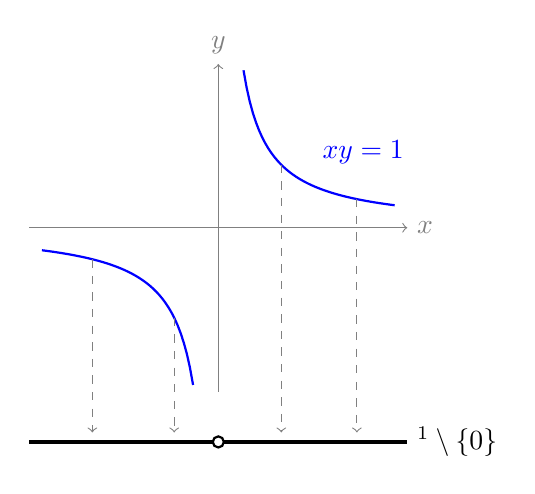
\begin{tikzpicture}[scale=0.8]
  \draw[->,gray] (-3,0)--(3,0) node[right]{$x$};
  \draw[->,gray] (0,-2.6)--(0,2.6) node[above]{$y$};
  \draw[thick,blue,domain=0.4:2.8,samples=50] plot (\x,{1/\x});
  \draw[thick,blue,domain=-2.8:-0.4,samples=50] plot (\x,{1/\x});
  \node[blue] at (2.3,1.2) {$xy=1$};
  \draw[very thick] (-3,-3.4)--(-0.07,-3.4);
  \draw[very thick] (0.07,-3.4)--(3,-3.4);
  \draw[thick,fill=white] (0,-3.4) circle (2.5pt);
  \node[right] at (3,-3.4) {$\A^1\setminus\{0\}$};
  \foreach \t in {-2,-0.7,1,2.2}{
    \draw[dashed,->,gray] (\t,{1/\t}) -- (\t,-3.25);
  }
\end{tikzpicture}
\caption{双曲線 $\Zero(xy-1)$ の $x$ 軸への射影は $\A^1\setminus\{0\}$ への同型．}
\label{fig:ch05-hyperbola}
\end{figure}

\begin{note}
すべての開集合がアフィンになるわけではない．例えば $\A^2\setminus\{0\}$ 上の正則関数は $k[x,y]$ に一致する（Hartogs 現象の代数版）ので，
もしアフィンなら $\A^2$ と同型になってしまうが，$\A^2\setminus\{0\}\to\A^2$ は全射でないので矛盾する．
\end{note}

\begin{myex}{尖点曲線：同相だが同型でない}{ch05-cusp}
$C=\Zero(y^2-x^3)$ とし，$\varphi:\A^1\to C$，$t\mapsto(t^2,t^3)$ を考える．
\begin{itemize}
  \item \textbf{全単射：} $(x,y)\in C$ で $x\neq0$ なら $t=y/x$ が唯一の逆像（$t^2=y^2/x^2=x$，$t^3=x t=y$），$x=0$ なら $y=0$ で $t=0$．
  \item \textbf{同相：} $\A^1$ と $C$ はともに既約な曲線であり，真の閉集合は有限集合のみである．全単射は有限集合を有限集合に移すので，$\varphi$ も $\varphi^{-1}$ も連続である．
  \item \textbf{同型でない：} 逆写像は $(x,y)\mapsto y/x$（$x\ne 0$），$(0,0)\mapsto0$ で与えられるが，これは多項式で書けない．
        実際，もし $\psi:C\to\A^1$ が射で $\psi\circ\varphi=\mathrm{id}$ なら，$\psi=G(\bar x,\bar y)$ として $G(t^2,t^3)=t$．
        しかし $G(t^2,t^3)\in k[t^2,t^3]$ は $t$ の1次の項をもたない（例 \ref{ex:ch05-coord-examples} (4)）ので矛盾する．
\end{itemize}
代数的には，$\varphi^*:k[C]\to k[\A^1]=k[t]$ の像が $k[t^2,t^3]\subsetneq k[t]$ で全射でないことが原因である．
幾何学的には，$C$ は原点に特異点をもつ（原点での接空間が2次元になる，第7章）のに対し $\A^1$ は滑らかである．
同相写像であっても局所的な代数構造（局所環，第6章）までは保たない．
\end{myex}

\begin{figure}[H]
\centering
\begin{tikzpicture}[scale=0.85]
  \draw[very thick] (-2.2,0)--(2.2,0) node[right]{$\A^1$};
  \foreach \t/\c in {-1.4/red,-0.7/orange,0/black,0.7/teal,1.4/blue}{\fill[\c] (\t,0) circle (2pt);}
  \draw[->,thick] (2.9,0)--(4.4,0) node[midway,above]{$t\mapsto(t^2,t^3)$};
  \begin{scope}[xshift=5.4cm]
    \draw[->,gray] (-0.5,0)--(2.6,0);
    \draw[->,gray] (0,-2)--(0,2);
    \draw[thick,red!70!black,domain=0:1.5,samples=60] plot ({\x*\x},{\x*\x*\x/1.2});
    \draw[thick,red!70!black,domain=0:1.5,samples=60] plot ({\x*\x},{-\x*\x*\x/1.2});
    \foreach \t/\c in {-1.4/red,-0.7/orange,0/black,0.7/teal,1.4/blue}{
      \fill[\c] ({\t*\t},{\t*\t*\t/1.2}) circle (2pt);}
    \node at (1.5,-2.3) {$C=\Zero(y^2-x^3)$};
  \end{scope}
\end{tikzpicture}
\caption{$\A^1$ から尖点曲線への全単射．逆写像は原点で多項式にならない．}
\label{fig:ch05-cusp}
\end{figure}

\subsection{多様体の埋め込み}

\begin{mydef}{閉埋め込み}{ch05-closed-emb}
射 $\varphi:X\to Y$ が\textbf{閉埋め込み}であるとは，像 $Z=\varphi(X)$ が $Y$ の閉集合であり，
$\varphi$ が $X$ から $Z$（閉部分多様体としての構造）への同型を与えることをいう．
\end{mydef}

\begin{myprop}{閉埋め込みの代数的判定}{ch05-closed-emb-crit}
アフィン代数的集合の射 $\varphi:X\to Y$ が閉埋め込みであるための必要十分条件は，$\varphi^*:k[Y]\to k[X]$，$g\mapsto g\circ\varphi$ が全射であることである．
\end{myprop}

\begin{proof}[証明の概略]
閉埋め込みなら $\varphi^*$ は制限写像 $k[Y]\to k[Z]$ と同型 $k[Z]\cong k[X]$ の合成であり，前者は全射（命題 \ref{prop:ch05-coord-ring} と同じ理由）．
逆に $\varphi^*$ が全射で核を $J$ とすると $k[X]\cong k[Y]/J$．$Z=\Zero_Y(J)$ とすると $k[Z]=k[Y]/\sqrt J=k[Y]/J$（$k[Y]/J\cong k[X]$ が被約なので $J$ は根基）．
次節の定理 \ref{thm:ch05-equiv} により，この $k$ 代数同型 $k[Z]\cong k[X]$ は同型 $X\cong Z$ から来ており，それが $\varphi$ と一致する．
\end{proof}

とくに，アフィン代数的集合 $X$ を座標環の生成元 $f_1,\dots,f_m$ を用いて写した $X\to\A^m$，$p\mapsto(f_1(p),\dots,f_m(p))$ は閉埋め込みである
（$k[y_1,\dots,y_m]\to k[X]$，$y_j\mapsto f_j$ が全射だから）．アフィン代数的集合とは「アフィン空間に閉埋め込みできる空間」であり，
埋め込み方は生成元の選び方だけある．

\begin{myex}{埋め込みの例}{ch05-emb-ex}
\begin{enumerate}
  \item $\A^1\to\A^3$，$t\mapsto(t,t^2,t^3)$ はねじれ3次曲線への閉埋め込み．$\varphi^*(x)=t$ なので全射．
  \item 射 $\varphi:X\to Y$ のグラフ $\Gamma_\varphi=\{(p,\varphi(p))\}\subset X\times Y$ への写像 $p\mapsto(p,\varphi(p))$ は閉埋め込み．
  \item 尖点曲線への $\varphi:\A^1\to C\subset\A^2$ は単射かつ像は閉だが，閉埋め込みではない（$\varphi^*$ が全射でない）．
  \item $\A^1\to\A^2$，$t\mapsto(t^2-1,\ t(t^2-1))$ は結節曲線 $\Zero(y^2-x^2(x+1))$ への全射だが，$t=\pm1$ が同じ点に移り単射でない．
\end{enumerate}
\end{myex}

\begin{physbox}[埋め込みとパラメータ表示]
物理では空間を「パラメータで表示する」（$\A^1\to C$）ことと「拘束条件で切り出す」（$C=\Zero(f)\subset\A^2$）ことの両方がよく用いられる．
前者は射 $\A^1\to C$，後者は閉埋め込み $C\hookrightarrow\A^2$ である．
尖点曲線の例は，パラメータ表示が全単射でも「良い座標」になっていないことがあることを示している．
例えば $t$ を時間とする粒子の軌道 $(x,y)=(t^2,t^3)$ は $t=0$ で速度が $0$ になって軌道が尖る．
曲線上の関数としては $t=y/x$ は滑らかに見えても，原点では多項式（あるいは正則関数）として表せない．
\end{physbox}

\exprob{prob:ch05-5-1}
$\varphi:\A^1\to\A^2$，$t\mapsto(t^2,t^5)$ の像を定める多項式を求め，$\varphi$ が像への同相写像であるが同型ではないことを示せ．

\exprob{prob:ch05-5-2}
$k=\C$ とする．$\A^1$ から $\A^1$ への同型はすべて $t\mapsto at+b$（$a\neq0$）の形であることを示せ．
また $\Zero(xy-1)$ の自己同型をすべて求めよ．

% ----------------------------------------------------------
\section{幾何学と環論の対応}
\label{sec:ch05-ring-geom}
% ----------------------------------------------------------

\subsection{多様体の射と環準同型}

射 $\varphi:X\to Y$ が与えられると，関数の引き戻し
\[
  \varphi^*:k[Y]\to k[X],\qquad \varphi^*(g)=g\circ\varphi
\]
が定まる．$g\in k[Y]$ が多項式 $G(y_1,\dots,y_m)$ の制限なら $g\circ\varphi$ は $G(F_1,\dots,F_m)$ の制限であって $k[X]$ に属し，
$\varphi^*$ が $k$ 代数準同型であること（和・積・定数を保つこと）は明らかである．
本章の中心定理は，逆にすべての $k$ 代数準同型がこのようにして得られることである．

\begin{mythm}{射と $k$ 代数準同型の対応}{ch05-morph-hom}
$X,Y$ をアフィン代数的集合とする．写像
\[
  \Hom(X,Y)\longrightarrow\Hom_{k\text{-alg}}(k[Y],k[X]),\qquad \varphi\longmapsto\varphi^*
\]
は全単射である．
\end{mythm}

\begin{proof}
$Y\subset\A^m$ とし，$k[Y]=k[y_1,\dots,y_m]/\Ideal(Y)$，$\bar y_j$ を座標関数とする．

\textbf{単射性．} $\varphi,\psi:X\to Y$ が $\varphi^*=\psi^*$ を満たすとする．各 $j$ について
$\bar y_j\circ\varphi=\varphi^*(\bar y_j)=\psi^*(\bar y_j)=\bar y_j\circ\psi$．
点 $\varphi(p)\in Y\subset\A^m$ はその座標 $(\bar y_1(\varphi(p)),\dots,\bar y_m(\varphi(p)))$ で決まるので $\varphi=\psi$．

\textbf{全射性．} $k$ 代数準同型 $u:k[Y]\to k[X]$ が与えられたとする．$f_j=u(\bar y_j)\in k[X]$ とおき
\[
  \varphi:X\to\A^m,\qquad \varphi(p)=(f_1(p),\dots,f_m(p))
\]
と定める．これは多項式写像である．像が $Y$ に含まれることを示す．$G\in\Ideal(Y)$ とすると，$u$ は $k$ 代数準同型なので
\[
  G(f_1,\dots,f_m)=G(u(\bar y_1),\dots,u(\bar y_m))=u\bigl(G(\bar y_1,\dots,\bar y_m)\bigr)=u(0)=0\quad(\text{in }k[X])．
\]
よって任意の $p\in X$ で $G(\varphi(p))=G(f_1,\dots,f_m)(p)=0$，すなわち $\varphi(p)\in\Zero(\Ideal(Y))=Y$．
こうして射 $\varphi:X\to Y$ を得た．最後に $\varphi^*=u$ を確かめる．
$\varphi^*(\bar y_j)=\bar y_j\circ\varphi=f_j=u(\bar y_j)$ であり，$k[Y]$ は $\bar y_j$ たちで $k$ 代数として生成されるので，
二つの $k$ 代数準同型 $\varphi^*$ と $u$ は一致する．
\end{proof}

証明の要点は，「$k[Y]$ からの準同型は生成元 $\bar y_j$ の行き先で決まり，行き先は関係式 $\Ideal(Y)$ を満たしさえすればよい」という商環の普遍性と，
「$X$ の点は $\Zero(\Ideal(Y))$ に入るかどうかで $Y$ の点か判定できる」という零点定理の帰結
（$Y=\Zero(\Ideal(Y))$）を組み合わせたことである．

\begin{myex}{対応の具体例}{ch05-morph-hom-ex}
\begin{enumerate}
  \item 点 $p:\{\mathrm{pt}\}\to X$ は $k[X]\to k[\mathrm{pt}]=k$，すなわち評価写像 $f\mapsto f(p)$ に対応する．
        よって $X\cong \Hom_{k\text{-alg}}(k[X],k)$．これは命題 \ref{prop:ch05-ideal-corr} の言い換えである（核が $\m_p$）．
  \item 射 $X\to\A^1$ は $k[t]\to k[X]$，すなわち $t$ の行き先 $f\in k[X]$ で決まる．よって $\Hom(X,\A^1)=k[X]$：
        \emph{座標環の元とは $\A^1$ への射のことである．}
  \item 尖点曲線のパラメータ表示 $\A^1\to C$ は $k[x,y]/(y^2-x^3)\to k[t]$，$x\mapsto t^2$，$y\mapsto t^3$ に対応する．
  \item 射影 $\Zero(xy-1)\to\A^1$ は包含 $k[x]\hookrightarrow k[x,x^{-1}]$ に対応する．
\end{enumerate}
\end{myex}

\subsection{反変性}

対応 $\varphi\mapsto\varphi^*$ は合成と整合的であるが，\emph{向きを逆にする}．
射 $X\xrightarrow{\varphi}Y\xrightarrow{\psi}Z$ に対して，$h\in k[Z]$ について
$(\psi\circ\varphi)^*(h)=h\circ\psi\circ\varphi=\varphi^*(\psi^*(h))$ なので
\[
  (\psi\circ\varphi)^*=\varphi^*\circ\psi^*,\qquad (\mathrm{id}_X)^*=\mathrm{id}_{k[X]}.
\]

\begin{figure}[H]
\centering
\begin{tikzcd}[column sep=large,row sep=large]
  X \arrow[r,"\varphi"] \arrow[rr,bend left=30,"\psi\circ\varphi"] & Y \arrow[r,"\psi"] & Z\\
  k[X] & k[Y] \arrow[l,"\varphi^*"'] & k[Z] \arrow[l,"\psi^*"'] \arrow[ll,bend left=30,"\varphi^*\circ\psi^*"]
\end{tikzcd}
\caption{座標環をとる操作は矢印の向きを逆にする（反変関手）．}
\end{figure}

この反変性から直ちに次がわかる．

\begin{mycor}{同型の判定}{ch05-iso-crit}
アフィン代数的集合 $X,Y$ について，$X\cong Y$ であることと $k[X]\cong k[Y]$（$k$ 代数として）であることは同値である．
より詳しく，射 $\varphi$ が同型であることと $\varphi^*$ が同型であることは同値である．
\end{mycor}

\begin{proof}
$\psi\circ\varphi=\mathrm{id}$，$\varphi\circ\psi=\mathrm{id}$ は $\varphi^*\circ\psi^*=\mathrm{id}$，$\psi^*\circ\varphi^*=\mathrm{id}$ と同値（定理 \ref{thm:ch05-morph-hom} の全単射性）．
また任意の $k$ 代数同型 $k[Y]\to k[X]$ はある射の引き戻しである．
\end{proof}

この系により，尖点曲線 $C$ と $\A^1$ が同型でないことは「$k[t^2,t^3]\not\cong k[t]$」に帰着される．
後者は例えば，$k[t]$ が整閉（UFD）であるのに $k[t^2,t^3]$ では $t=t^3/t^2$ が商体の元として整（$t^2-\bar x=0$ の根）だが環に属さない，ことから分かる．

圏論の言葉でまとめよう（圏論的視点の一般論は第10章で改めて扱う）．

\begin{mythm}{アフィン代数的集合と $k$ 代数の反変同値}{ch05-equiv}
関手
\[
  \left\{\begin{array}{c}\text{アフィン代数的集合}\\ \text{と射}\end{array}\right\}
  \longrightarrow
  \left\{\begin{array}{c}\text{有限生成被約 } k \text{ 代数}\\ \text{と } k \text{ 代数準同型}\end{array}\right\}^{\mathrm{op}}
\]
（$X\mapsto k[X]$，$\varphi\mapsto\varphi^*$）は圏同値である．この同値はアフィン多様体（既約）の圏と有限生成整域 $k$ 代数の圏の反対圏との同値に制限される．
\end{mythm}

\begin{proof}
圏同値であるためには，関手が忠実充満であり，かつ本質的全射（任意の対象が像のある対象と同型）であればよい．
忠実充満性は定理 \ref{thm:ch05-morph-hom}，本質的全射性は命題 \ref{prop:ch05-fg-reduced} の後半である．
既約な場合への制限は命題 \ref{prop:ch05-domain} による．
\end{proof}

逆向きの関手（擬逆）は，$A$ に対して生成元を選んで $A\cong k[x_1,\dots,x_n]/I$ と表示し，$X_A=\Zero(I)$ を対応させるものである．
生成元の選び方によって $X_A$ は異なる $\A^n$ に入るが，系 \ref{cor:ch05-iso-crit} によりすべて互いに（標準的に）同型である．

\subsection{幾何学的対象の代数的記述}

反変同値のおかげで，アフィン幾何のほぼすべての概念を座標環の言葉に翻訳できる．代表的なものを表にまとめる．

\begin{center}
\renewcommand{\arraystretch}{1.35}
\begin{tabular}{l|l}
幾何（アフィン代数的集合） & 代数（有限生成被約 $k$ 代数）\\ \hline
$X$ & $k[X]$\\
点 $p\in X$ & 極大イデアル $\m_p$／準同型 $k[X]\to k$\\
閉部分集合 $Z\subset X$ & 根基イデアル $J$（$k[Z]=k[X]/J$）\\
既約閉部分集合 & 素イデアル\\
射 $\varphi:X\to Y$ & $k$ 代数準同型 $\varphi^*:k[Y]\to k[X]$\\
同型 & $k$ 代数同型\\
閉埋め込み & 全射準同型\\
支配的な射（像が稠密） & 単射準同型\\
直積 $X\times Y$ & テンソル積 $k[X]\otimes_k k[Y]$\\
$X\to\A^1$ & $k[X]$ の元\\
基本開集合 $D(f)=\{f\neq0\}$ & 局所化 $k[X]_f$（第6章）\\
点 $p$ の近傍での関数の芽 & 局所環 $\OO_{X,p}=k[X]_{\m_p}$（第6章）
\end{tabular}
\end{center}

「支配的 $\iff$ 単射」を確かめておく．$g\in\Ker\varphi^*$ とは $g\circ\varphi=0$，すなわち $g$ が $\varphi(X)$ 上 $0$ ということであり，
$\Ker\varphi^*=\Ideal_Y(\varphi(X))$．これが $0$ であることは $\overline{\varphi(X)}=\Zero_Y(\Ideal_Y(\varphi(X)))=Y$ と同値である．
例えば $\A^2\to\A^2$，$(x,y)\mapsto(x,xy)$ の像は $\{x\neq 0\}\cup\{(0,0)\}$ で閉集合でも開集合でもないが稠密であり，
$k[u,v]\to k[x,y]$，$u\mapsto x,\ v\mapsto xy$ は単射である．このように射の像は閉とは限らない
（像は構成可能集合になる，という Chevalley の定理がある）．

直積 $X\times Y\subset\A^{n+m}$ について $k[X\times Y]\cong k[X]\otimes_kk[Y]$ が成り立つ（$k$ が代数閉体であることを使う）．
例えば $k[\A^n\times\A^m]=k[x_1,\dots,x_n]\otimes_kk[y_1,\dots,y_m]=k[x,y]=k[\A^{n+m}]$．
ただし前に注意したように，$X\times Y$ の Zariski 位相は積位相ではない．

\subsection{座標環から多様体を理解する}

反変同値の実用的な意味は，「多様体についての問題を環についての問題に翻訳して計算できる」ことである．
また逆に，環論的な構成から新しい多様体を作ることができる．代表的な例が商である．

\begin{myex}{有限群による商：$\A^2/\{\pm1\}$}{ch05-quotient}
群 $G=\{\pm1\}$ を $\A^2$ に $(x,y)\mapsto(-x,-y)$ で作用させる．「軌道空間 $\A^2/G$」を代数多様体として作りたい．
$G$ 不変な関数のなす部分環
\[
  k[x,y]^G=k[x^2,\ xy,\ y^2]
\]
は有限生成整域であり，生成元 $u=x^2,\ v=y^2,\ w=xy$ の間の関係は $uv=w^2$ で尽きる．したがって
\[
  \A^2/G:=\text{（$k[x,y]^G$ に対応する多様体）}=\Zero(uv-w^2)\subset\A^3
\]
は二次錐面である．包含 $k[x,y]^G\hookrightarrow k[x,y]$ に対応する射 $\A^2\to\Zero(uv-w^2)$，$(x,y)\mapsto(x^2,y^2,xy)$ は全射で，
各ファイバーがちょうど一つの $G$ 軌道になる．原点の像（錐の頂点）は特異点である．
\end{myex}

ここでは「軌道空間」という位相的な構成を直接行うのではなく，\emph{不変式環をとる}という代数的操作で商を定義した．
これは座標環から多様体を作るという発想の典型的な応用であり，幾何学的不変式論（GIT）の出発点である．

\begin{physbox}[真空のモジュライ空間とカイラル環]
超対称ゲージ理論では，古典的な真空のモジュライ空間は「スカラー場の配位空間をゲージ群で割ったもの」であり，
実際の計算ではゲージ不変な正則多項式（カイラル演算子）の環を求め，その間の関係式を調べる．
例えば $U(1)$ ゲージ理論で電荷 $+1$ の場 $\phi_+$ と $-1$ の場 $\phi_-$ があるとき，
ゲージ不変量は $M=\phi_+\phi_-$ で生成され，D 項条件を込めたモジュライ空間は $\Spec\,\C[M]\cong\A^1$ となる．
また $\C^2/\Z_2$ オービフォールド上の弦理論や，4次元 $\mathcal N=2$ の $U(1)$ ゲージ理論に電荷 $1$ のハイパー多重項を2つ入れた理論の Higgs ブランチ
では例 \ref{ex:ch05-quotient} の二次錐面 $uv=w^2$ がそのまま現れる．
「モジュライ空間 $=$ カイラル環に対応するアフィン多様体」という見方は，本章の反変同値の物理的実例である．
特異点（錐の頂点）では余分な無質量粒子が現れるなど物理的に特別なことが起き，第7章でその代数的な扱いを学ぶ．
\end{physbox}

最後に注意をひとつ．反変同値は「有限生成被約 $k$ 代数」に限定されていた．
任意の可換環 $R$（$\Z$ や $k[x]/(x^2)$ など）に対しても対応する幾何学的対象を考えたい，という要請から
スキーム $\Spec R$ が生まれる（第12章）．本章の定理 \ref{thm:ch05-equiv} は
「アフィンスキームの圏 $\simeq$ 可換環の圏の反対圏」という定理の古典的な特別の場合である．

\exprob{prob:ch05-6-1}
$\varphi:\A^2\to\A^2$，$(x,y)\mapsto(x,\ y+x^2)$ が同型であることを，$\varphi^*$ の逆写像を具体的に構成することで示せ．
さらに $\A^2$ の自己同型群が無限次元である（多項式 $g(x)$ ごとに $(x,y)\mapsto(x,y+g(x))$ が自己同型になる）ことを確かめよ．

\exprob{prob:ch05-6-2}
$G=\Z/3\Z$ を $\A^2_\C$ に $(x,y)\mapsto(\omega x,\omega^2y)$（$\omega=e^{2\pi i/3}$）で作用させる．
不変式環 $\C[x,y]^G$ の生成元と関係式を求め，商 $\A^2/G$ が $\A^3$ のどのような曲面として実現されるかを答えよ．

\section*{問題の解答}
\addcontentsline{toc}{section}{問題の解答}

\exsol{prob:ch05-1-1}
$I=(x^2-yz,\ xz-x)$ とおく．$xz-x=x(z-1)$ なので，$X$ の点は $x=0$ または $z=1$ を満たす．
$x=0$ のとき $yz=0$ なので $y=0$ または $z=0$．$z=1$ のとき $y=x^2$．よって
\[
  X=L_1\cup L_2\cup C,
\]
\[
  L_1=\Zero(x,y)\ (z\text{ 軸}),\qquad L_2=\Zero(x,z)\ (y\text{ 軸}),\qquad C=\Zero(z-1,\ y-x^2).
\]
$C$ は平面 $z=1$ 上の放物線である．
$L_1,L_2,C$ はそれぞれ $\A^1$ と同型（$z\mapsto(0,0,z)$，$y\mapsto(0,y,0)$，$t\mapsto(t,t^2,1)$）なので既約であり，
$(0,0,1)\in L_1\setminus(L_2\cup C)$ のような点を見れば互いに他を含まないので，これが既約成分分解である．

\textbf{各成分の消滅イデアル．}
\[
  \Ideal(L_1)=(x,y),\qquad\Ideal(L_2)=(x,z),\qquad\Ideal(C)=(z-1,\ y-x^2).
\]
例えば $f\in\Ideal(C)$ なら，$z=1+(z-1)$，$y=x^2+(y-x^2)$ と書き換えて $f=(z-1)g_1+(y-x^2)g_2+h(x)$ とでき，$h(t)=f(t,t^2,1)=0$ が全ての $t$ で成り立つので $h=0$．
$L_1,L_2$ についても同様である．剰余環はそれぞれ $k[z],k[y],k[x]$ で整域なので，いずれも素イデアルである．

\textbf{共通部分が $\Ideal(X)$ に等しいこと．}
$P=\Ideal(L_1)\cap\Ideal(L_2)\cap\Ideal(C)$ とおく．$\Ideal$ は和集合を共通部分に写すので（第4章の命題，消滅イデアルの性質）$P=\Ideal(X)$ であるが，ここでは実際に
\[
  I\subset P\subset I,\qquad\text{すなわち}\quad \Ideal(X)=P=I=(x^2-yz,\ xz-x)
\]
となることを確かめる．
$I\subset P$：$x^2-yz$ と $x(z-1)$ は $(x,y)$，$(x,z)$ に属し，$z=1,\ y=x^2$ を代入すると $0$ になるので $(z-1,y-x^2)$ にも属する．

$P\subset I$：まず $yz(z-1)=-(z-1)(x^2-yz)+x\cdot x(z-1)\in I$ に注意する．
$I$ を法として $x^2\equiv yz$，$xz\equiv x$，$yz^2\equiv yz$ という書き換えを繰り返すと（各書き換えで $x$ の次数か $z$ の次数が下がるので有限回で止まる），
任意の多項式は $I$ を法として
\[
  r=x\,p(y)+u(z)+y\,q(y)+yz\,s(y)\qquad(p,q,s\in k[y],\ u\in k[z])
\]
の形の多項式と合同になる（$x^2$，$xz$，$yz^2$ で割り切れる単項式が残らない形）．
$f\in P$ とし，$f\equiv r\pmod I$ とする．$I\subset P$ なので $r\in P$，すなわち $r$ は $X$ 上で消える．
\begin{itemize}
  \item $L_1$ 上 $(0,0,z)$：$r=u(z)=0$ が全ての $z$ で成り立つので $u=0$．
  \item $L_2$ 上 $(0,y,0)$：$r=y\,q(y)=0$ より $q=0$．
  \item $C$ 上 $(t,t^2,1)$：$r=t\,p(t^2)+t^2s(t^2)=0$．第1項は奇数次，第2項は偶数次の項のみなので $p=s=0$．
\end{itemize}
よって $r=0$，$f\in I$．以上で $\Ideal(X)=(x,y)\cap(x,z)\cap(z-1,y-x^2)=(x^2-yz,\ xz-x)$ が示された．
特に，$X$ を定義する方程式 $x^2-yz,\ xz-x$ はすでに根基イデアルを生成している．

\exsol{prob:ch05-1-2}
\textbf{$\A^1$ の無限部分集合は稠密．}
$\A^1$ の閉集合は $\Zero(S)$ の形であり，$S$ が零でない多項式 $f$ を含めば $\Zero(S)\subset\Zero(f)$ は高々 $\deg f$ 個の点からなる有限集合である．
したがって $\A^1$ の閉集合は有限集合か $\A^1$ 自身に限る．無限部分集合 $T$ の閉包 $\overline T$ は $T$ を含む閉集合なので無限集合，よって $\overline T=\A^1$．

\textbf{$\A^2$ の Zariski 位相は積位相と異なる．}
対角線 $\Delta=\Zero(x-y)\subset\A^2$ は Zariski 閉集合である．$\Delta$ が積位相で閉でないことを示す．
積位相で閉だとすると，補集合 $U=\A^2\setminus\Delta$ は積位相の開集合なので，点 $(0,1)\in U$ に対し，$\A^1$ の空でない開集合 $U_1,U_2$ で $(0,1)\in U_1\times U_2\subset U$ となるものがある．
上で見たように $U_1,U_2$ は有限集合の補集合なので，$U_1\cap U_2$ も有限集合の補集合であり，$k$ は無限体だから空でない．
$c\in U_1\cap U_2$ をとると $(c,c)\in U_1\times U_2\subset U$ となり，$(c,c)\in\Delta$ に矛盾．
よって $\Delta$ は積位相で閉でなく，Zariski 位相は積位相より真に細かい．
（積位相の閉集合は「有限個の点と有限個の縦横の直線の和」の共通部分からなり，$\Delta$ や放物線のような曲線は含まれない．）

\exsol{prob:ch05-2-1}
\textbf{$xy-z^2$ の既約性．}
$F=xy-z^2$ を $k[y,z][x]$ の元とみると $x$ について1次で，$F=y\cdot x-z^2$．$F=GH$ と分解したとすると，$x$ についての次数から一方，例えば $H$ は $x$ を含まず，
$G=G_1x+G_0$（$G_i\in k[y,z]$）として $HG_1=y$，$HG_0=-z^2$．よって $H$ は $y$ と $z^2$ の公約元であり，$\gcd(y,z^2)=1$ なので $H$ は定数．
したがって $F$ は既約である．$k[x,y,z]$ は UFD なので $(F)$ は素イデアルであり，特に根基なので零点定理より $\Ideal(X)=(F)$ は素イデアル，$X$ はアフィン多様体である．

\textbf{$k[X]$ は UFD でない．}
$A=k[X]=k[x,y,z]/(xy-z^2)$ とする．$F$ は斉次なので $A$ は次数付き環 $A=\bigoplus_{d\ge0}A_d$，$A_0=k$ となり，$A$ は整域である．
\begin{itemize}
  \item \emph{単元は $k^\times$ のみ．}$ab=1$ とし，$a,b$ の最高次の斉次成分を $a_m,b_n$ とすると，整域なので $a_mb_n\ne0$ が $ab$ の $m+n$ 次成分になる．$ab=1$ より $m+n=0$，$m=n=0$，すなわち $a,b\in k^\times$．
  \item \emph{1次の斉次元 $\ell\ne0$ は既約．}$\ell=ab$ なら同様に最高次の次数の和が $1$ なので，一方の最高次は $0$，すなわちそれは $A_0=k$ に属する定数であり，単元である．また $\ell$ は次数 $1$ なので単元でない．
\end{itemize}
$\bar x,\bar y,\bar z$ はいずれも $0$ でない（$x,y,z$ は2次式 $F$ の倍数でない）1次元なので既約元である．
そして $A$ において
\[
  \bar z\cdot\bar z=\bar x\cdot\bar y
\]
は既約元への二通りの分解を与える．これらが本質的に異なることを見るには，$\bar z$ が $\bar x$ に同伴でないことを示せばよい：$\bar z=c\bar x$（$c\in k^\times$）なら $z-cx\in(F)$ だが，零でない1次式は2次式 $F$ の倍数になりえない．
$\bar z$ と $\bar y$ についても同様．よって分解は一意でなく，$A$ は UFD でない．
（同じことだが，$\bar z$ は既約元なのに $\bar z\mid\bar x\bar y$，$\bar z\nmid\bar x$，$\bar z\nmid\bar y$ なので素元でない．）
幾何学的には，直線 $\Zero_X(\bar x)=\{x=z=0\}$ は錐面 $X$ 上で「1本の方程式で切り出されない」ことに対応している（$\bar x=0$ で切ると直線が二重に現れる）．

\exsol{prob:ch05-3-1}
\textbf{$\Zero(J)$ の既約分解．}
$\Zero(J)$ の点では $y=x^2$ なので $xz-y^2=xz-x^4=x(z-x^3)$．したがって $x=0$（このとき $y=0$，$z$ は任意）または $z=x^3$ であり，
\[
  \Zero(J)=C\cup L,\qquad L=\Zero(x,y)\ (z\text{ 軸}),\quad C=\Zero(y-x^2,\ z-x^3).
\]
$L\cong\A^1$，$C\cong\A^1$ はともに既約である．$(0,0,1)\in L$ だが $(0,0,1)\notin C$（$z=1\ne0=x^3$）なので $L\not\subset C$，
また $(1,1,1)\in C\setminus L$ なので $C\not\subset L$．よってこれが既約成分分解であり，特に $\Zero(J)\supsetneq C$．
$\Zero$ と $\Ideal$ の対応から $J\subset\Ideal(\Zero(J))\subsetneq\Ideal(C)$ なので $J\ne\Ideal(C)$．
（例えば $z-x^3\in\Ideal(C)$ は $(0,0,1)$ で消えないので $J$ に属さない．）

\textbf{追加すべき方程式．}
$L$ 上で消えずに $C$ 上で消える方程式を一つ加えればよい．例えば $z-x^3$ を加えると
\[
  J+(z-x^3)=(xz-y^2,\ y-x^2,\ z-x^3)=(y-x^2,\ z-x^3)=\Ideal(C)
\]
となる．実際 $xz-y^2=x(z-x^3)-(y-x^2)(y+x^2)$ なので $xz-y^2$ は不要になり，最後の等号は第4章の問4.5.1で示した．
ねじれ3次曲線の標準的な方程式系 $y-x^2,\ z-xy,\ xz-y^2$ のように $z-xy$ を加えてもよい（$y=x^2$ のもとで $z-xy=z-x^3$）．
$y-x^2$ と $xz-y^2$ だけでは，$x=0$ のとき $z$ についての情報が失われ，余分な直線 $L$ が現れるのである．

\exsol{prob:ch05-4-1}
$A=k[x,y]/(x^2,xy)$ は $\bar x,\bar y$ で生成されるので有限生成 $k$ 代数である．
$(x^2,xy)$ の元は1次以下の項をもたないので $x\notin(x^2,xy)$，すなわち $\bar x\ne0$．一方 $\bar x^2=0$ なので $\bar x$ は $0$ でない冪零元であり，$A$ は被約でない．

\textbf{冪零根基．}
第4章の根基の計算例で見たように $\sqrt{(x^2,xy)}=(x)$（$x^2\in(x^2,xy)$ より $(x)\subset\sqrt{(x^2,xy)}$，$(x^2,xy)\subset(x)$ で $(x)$ は素なので逆の包含）．
したがって $A$ の冪零根基は
\[
  \sqrt{0_A}=(x)/(x^2,xy)=\bar xA=k\,\bar x
\]
である．最後の等号は，$\bar x\bar x=0$，$\bar x\bar y=0$ なので $\bar x\cdot f=f(0,0)\,\bar x$ となることによる．冪零根基は $\bar x$ で張られる1次元の $k$ ベクトル空間である．

\textbf{座標環．}
$\Zero(x^2,xy)=\Zero(x)$ は $y$ 軸であり，零点定理より $\Ideal(\Zero(x^2,xy))=\sqrt{(x^2,xy)}=(x)$．よって
\[
  k[\Zero(x^2,xy)]=k[x,y]/(x)\cong k[y]\cong A/\sqrt{0_A}.
\]
命題\ref{prop:ch05-coord-def-ideal}の通り，自然な全射 $A\to k[\Zero(x^2,xy)]$ の核がちょうど冪零根基 $k\bar x$ である．
失われた $\bar x$ は，原点に埋め込まれた「$x$ 方向の無限小の厚み」（第4章の図の埋没点）を表している．

\exsol{prob:ch05-5-1}
\textbf{像の方程式．}
$C=\Zero(y^2-x^5)$ とおく．$(t^5)^2=(t^2)^5$ なので $\varphi(\A^1)\subset C$．
逆に $(a,b)\in C$ とする．$a=0$ なら $b=0=\varphi(0)$．$a\ne0$ なら $t=b/a^2$ とおくと $t^2=b^2/a^4=a$，$t^5=t\cdot(t^2)^2=(b/a^2)a^2=b$．
よって $\varphi(\A^1)=C$．また $\varphi(t)=\varphi(t')$ なら，$t\neq0$ のとき $t=t^5/t^4=y/x^2$ が像から決まり，$t=0$ は原点のみに写るので $\varphi$ は単射．
$y^2-x^5$ は既約（$y$ についてモニック2次式なので，分解すれば $a(x)^2=x^5$ となる $a$ があることになるが次数の偶奇から不可能）なので $(y^2-x^5)$ は素イデアルであり，
$\Ideal(C)=(y^2-x^5)$．すなわち像は方程式 $y^2=x^5$ で定まる．

\textbf{$\varphi^*$ の計算．}
$\varphi^*\colon k[x,y]\to k[t]$，$x\mapsto t^2$，$y\mapsto t^5$ の核は $(y^2-x^5)$ である．実際 $f$ を $y$ についてのモニック多項式 $y^2-x^5$ で割って $f\equiv a(x)+b(x)y$ とすると，
$\varphi^*(f)=a(t^2)+b(t^2)t^5$ は偶数次の部分 $a(t^2)$ と奇数次の部分 $b(t^2)t^5$ に分かれるので，$0$ になるのは $a=b=0$ のときに限る．
よって $\varphi^*\colon k[C]\to k[t]$ は単射で，像は $k[t^2,t^5]$，すなわち $t^{2i+5j}$ の張る空間である．$2i+5j$ の形に書けない非負整数は $1$ と $3$ のみなので
\[
  \varphi^*(k[C])=k[t^2,t^5]=\Bigl\{\sum_n c_nt^n\ \Big|\ c_1=c_3=0\Bigr\}\subsetneq k[t].
\]

\textbf{同相であること．}
$C$ の真の閉集合は有限集合であることを示す．$C\cap\Zero(g)$（$g\notin\Ideal(C)$）について，$\varphi^*(g)=g(t^2,t^5)$ は上の単射性より零でない多項式なので，
$\varphi^{-1}(C\cap\Zero(g))$ はその有限個の根からなり，$\varphi$ が全単射なので $C\cap\Zero(g)$ も有限．$C$ の閉集合はこうした集合の共通部分なので，$C$ 自身か有限集合である．
$\A^1$ の閉集合も $\A^1$ 自身か有限集合である（問\ref{prob:ch05-1-2}）．全単射 $\varphi$ は有限集合を有限集合に，全体を全体に写すので，$\varphi$ と $\varphi^{-1}$ はともに閉集合を閉集合に写す．よって $\varphi\colon\A^1\to C$ は同相写像である．

\textbf{同型でないこと．}
$\varphi$ が同型なら，系\ref{cor:ch05-iso-crit}により $\varphi^*\colon k[C]\to k[t]$ は同型，特に全射でなければならない．しかし $t\notin k[t^2,t^5]$ なので全射でない．
よって $\varphi$ は同型でない．具体的には，逆写像 $(x,y)\mapsto y/x^2$（原点では $0$）は原点で多項式で書けない．
これは尖点曲線（例\ref{ex:ch05-cusp}）と同じ現象であり，$C$ は原点に特異点（$(2,5)$ 型の尖点）をもつ．

\exsol{prob:ch05-5-2}
\textbf{$\A^1$ の自己同型．}
系\ref{cor:ch05-iso-crit}と定理\ref{thm:ch05-morph-hom}により，射 $\varphi\colon\A^1\to\A^1$ は $f=\varphi^*(t)\in k[t]$ で決まり $\varphi(c)=f(c)$ であって，$\varphi$ が同型であることと $\varphi^*$ が $k[t]$ の $k$ 代数自己同型であることは同値である．
$\varphi$ が同型で逆を $\psi$，$g=\psi^*(t)$ とすると，$(\psi\circ\varphi)^*=\varphi^*\circ\psi^*$ より
\[
  t=\varphi^*(\psi^*(t))=\varphi^*(g(t))=g(f(t)).
\]
$f$ が定数なら右辺も定数なので不可．$f,g$ がともに定数でなければ $\deg g(f(t))=\deg g\cdot\deg f$ であり，これが $1$ なので $\deg f=1$，すなわち $f=at+b$（$a\ne0$）．
逆に $t\mapsto at+b$（$a\ne0$）は逆写像 $t\mapsto(t-b)/a$ をもつ同型である．よって $\Aut(\A^1)=\{t\mapsto at+b\mid a\in k^\times,\ b\in k\}$（アフィン変換群）．

\textbf{$H=\Zero(xy-1)$ の自己同型．}
$k[H]=k[x,y]/(xy-1)\cong k[t,t^{-1}]$（$x\mapsto t$，$y\mapsto t^{-1}$）であり，$H$ の自己同型は $k[t,t^{-1}]$ の $k$ 代数自己同型 $\sigma$ と一対一に対応する．
\begin{itemize}
  \item \emph{単元の決定．}$k[t,t^{-1}]$ の単元は $ct^n$（$c\in k^\times$，$n\in\Z$）に限る．実際 $uv=1$ とし，$u=t^mu_0$，$v=t^lv_0$（$u_0,v_0\in k[t]$ は $t$ で割り切れない多項式）と書くと $u_0v_0=t^{-m-l}$ であり，左辺は $t$ で割り切れない多項式なので $m+l=0$，$u_0v_0=1$，よって $u_0,v_0\in k^\times$．
  \item $t$ は単元なので $\sigma(t)$ も単元であり，$\sigma(t)=ct^n$．$\sigma$ の像は $k[t^n,t^{-n}]$ であり，全射であるためには $t$ がこれに含まれなければならないので $n=\pm1$．
  \item 逆に $\sigma(t)=ct$ と $\sigma(t)=ct^{-1}$（$c\in k^\times$）はいずれも自己同型である（逆はそれぞれ $t\mapsto c^{-1}t$，$t\mapsto ct^{-1}$）．
\end{itemize}
$\sigma=\varphi^*$ に対応する射 $\varphi$ は $\varphi=(\sigma(\bar x),\sigma(\bar y))$ で与えられるので，$H$ の自己同型は
\[
  (x,y)\longmapsto(cx,\ c^{-1}y),\qquad (x,y)\longmapsto(cy,\ c^{-1}x)\qquad(c\in\C^\times)
\]
で尽きる．前者は $\C^\times$ の掛け算 $u\mapsto cu$，後者は $u\mapsto c/u$ であり，$\Aut(H)\cong\C^\times\rtimes\Z/2\Z$ である．
$\A^1$ と違って平行移動に相当するものがないのは，$H\cong\A^1\setminus\{0\}$ の「穴」が保たれなければならないからである．

\exsol{prob:ch05-6-1}
$\A^2$ の座標を，定義域側で $(x,y)$，値域側で $(u,v)$ とすると，$\varphi^*\colon k[u,v]\to k[x,y]$ は $u\mapsto x$，$v\mapsto y+x^2$ である．
$k$ 代数準同型 $\tau\colon k[x,y]\to k[u,v]$ を $x\mapsto u$，$y\mapsto v-u^2$ で定めると，生成元について
\[
  \tau(\varphi^*(u))=\tau(x)=u,\quad \tau(\varphi^*(v))=\tau(y+x^2)=(v-u^2)+u^2=v,
\]
\[
  \varphi^*(\tau(x))=\varphi^*(u)=x,\quad \varphi^*(\tau(y))=\varphi^*(v-u^2)=(y+x^2)-x^2=y.
\]
$k$ 代数準同型は生成元の行き先で決まるので $\tau\circ\varphi^*=\mathrm{id}$，$\varphi^*\circ\tau=\mathrm{id}$．よって $\varphi^*$ は同型であり，系\ref{cor:ch05-iso-crit}により $\varphi$ は同型である．
逆写像は $\tau=\psi^*$ となる射 $\psi(u,v)=(u,\ v-u^2)$ である．

全く同じ計算で，任意の $g(x)\in k[x]$ に対し $\varphi_g(x,y)=(x,\ y+g(x))$ は $\varphi_{-g}$ を逆とする同型である．さらに
\[
  \varphi_g\circ\varphi_h(x,y)=\varphi_g(x,\ y+h(x))=(x,\ y+h(x)+g(x))=\varphi_{g+h}(x,y)
\]
であり，$g\ne h$ なら $\varphi_g\ne\varphi_h$（点 $(c,0)$ の像は $(c,g(c))$ なので，$\varphi_g$ から $g$ の値がすべて読み取れる）．
よって $g\mapsto\varphi_g$ は加法群 $(k[x],+)$ から $\Aut(\A^2)$ への単射準同型である．$k[x]$ は $k$ 上無限次元のベクトル空間であり，$g$ の係数を自由に（任意に多く）とれるので，
$\Aut(\A^2)$ は有限個のパラメータでは記述できない「無限次元」の群である．
これは $\Aut(\A^1)$（2パラメータ）や $\GL_2$ のような有限次元の代数群と対照的である（$\Aut(\A^2)$ はこうした三角型の自己同型とアフィン変換で生成されることが知られている：Jung--van der Kulk の定理）．

\exsol{prob:ch05-6-2}
$G$ の生成元 $\sigma$ は $\sigma^*(x)=\omega x$，$\sigma^*(y)=\omega^2y$ と作用するので，単項式は
\[
  x^ay^b\longmapsto\omega^{a+2b}x^ay^b=\omega^{a-b}x^ay^b\qquad(\omega^3=1)
\]
と変換される．多項式 $f=\sum c_{ab}x^ay^b$ が不変であることは，各単項式の係数について $c_{ab}(\omega^{a-b}-1)=0$ であること，すなわち $c_{ab}\ne0$ なら $a\equiv b\pmod3$ であることと同値である．

\textbf{生成元．}
$u=x^3$，$v=y^3$，$w=xy$ はいずれも不変である．$a\equiv b\pmod 3$ なる単項式は，$a\ge b$ なら $a=b+3m$ として $x^ay^b=(xy)^b(x^3)^m=w^bu^m$，$a<b$ なら同様に $w^av^m$ と書ける．よって
\[
  \C[x,y]^G=\C[u,v,w]=\C[x^3,\ y^3,\ xy].
\]

\textbf{関係式．}
$uv=x^3y^3=w^3$ である．これで関係式が尽きることを示す．$\pi\colon\C[U,V,W]\to\C[x,y]^G$，$U\mapsto x^3$，$V\mapsto y^3$，$W\mapsto xy$ とする．
$UV$ を $W^3$ に置き換えることを繰り返すと，任意の多項式は $(UV-W^3)$ を法として，$U$ と $V$ を同時に含まない単項式 $U^iW^j$，$V^lW^j$（$i\ge0$，$l\ge1$）の一次結合と合同になる．
これらの像 $x^{3i+j}y^j$，$x^jy^{3l+j}$ はすべて相異なる単項式である（指数の差 $a-b$ が $3i\ge0$ か $-3l<0$ かで型が分かれ，$\min(a,b)=j$ と $a-b$ から $(i,j)$ または $(l,j)$ が決まる）ので一次独立である．
したがってそのような一次結合の像が $0$ なら係数はすべて $0$ であり，$\Ker\pi=(UV-W^3)$．よって
\[
  \C[x,y]^G\cong\C[U,V,W]/(UV-W^3).
\]

\textbf{商の実現．}
商 $\A^2/G$ は曲面
\[
  \A^2/G\cong\Zero(uv-w^3)\subset\A^3
\]
として実現され，商写像は $(x,y)\mapsto(x^3,y^3,xy)$ である．
$uv-w^3$ の偏微分 $(v,u,-3w^2)$ は原点でのみ同時に $0$ になるので，原点（$\A^2$ の原点，すなわち $G$ の固定点の像）がただ一つの特異点である．
これは $A_2$ 型の Du Val 特異点（Klein 特異点 $\C^2/\Z_3$）であり，例\ref{ex:ch05-quotient}の二次錐面 $uv=w^2$（$A_1$ 型，$\C^2/\Z_2$）の一般化である．
一般に $\Z/n\Z$ が $(x,y)\mapsto(\zeta x,\zeta^{-1}y)$ で作用すれば商は $uv=w^n$（$A_{n-1}$ 型）となる．
